% LyX 2.3.4.2 created this file.  For more info, see http://www.lyx.org/.
%% Do not edit unless you really know what you are doing.
% \documentclass[english,dvipsnames,aspectratio=169,handout]{beamer}
\documentclass[english,dvipsnames,aspectratio=169]{beamer}
\usepackage{mathptmx}
\usepackage{eulervm}
\usepackage[T1]{fontenc}
\usepackage[latin9]{inputenc}
\usepackage{babel}
\usepackage{amstext}
\usepackage{amssymb}
\usepackage{graphicx}
\usepackage{ifthen}
\usepackage{xcolor}
\usepackage{xspace}
\usepackage{tikz}
\usetikzlibrary{tikzmark}
\usetikzlibrary{calc}
\usetikzlibrary{positioning}
\usepackage{pgfplots}
%\pgfplotsset{compat=1.17}
\usepackage{booktabs}
\usepackage{xpatch}
\usepackage{multirow}
\usepackage{colortbl}
\usepackage{pgfpages}

\xpatchcmd{\itemize}
  {\def\makelabel}
  {\ifnum\@itemdepth=1\relax
     \setlength\itemsep{2ex}% separation for first level
   \else
     \ifnum\@itemdepth=2\relax
       \setlength\itemsep{1ex}% separation for second level
     \else
       \ifnum\@itemdepth=3\relax
         \setlength\itemsep{0.5ex}% separation for third level
   \fi\fi\fi\def\makelabel
  }
 {}
 {}

\ifx\hypersetup\undefined
  \AtBeginDocument{%
    \hypersetup{unicode=true,pdfusetitle,
 bookmarks=true,bookmarksnumbered=false,bookmarksopen=false,
 breaklinks=false,pdfborder={0 0 0},pdfborderstyle={},backref=false,colorlinks=true,
 allcolors=NYUPurple,urlcolor=LightPurple}
  }
\else
  \hypersetup{unicode=true,pdfusetitle,
 bookmarks=true,bookmarksnumbered=false,bookmarksopen=false,
 breaklinks=false,pdfborder={0 0 0},pdfborderstyle={},backref=false,colorlinks=true,
 allcolors=NYUPurple,urlcolor=LightPurple}
\fi

\makeatletter

%%%%%%%%%%%%%%%%%%%%%%%%%%%%%% LyX specific LaTeX commands.
%% Because html converters don't know tabularnewline
\providecommand{\tabularnewline}{\\}

%%%%%%%%%%%%%%%%%%%%%%%%%%%%%% Textclass specific LaTeX commands.
% this default might be overridden by plain title style
\newcommand\makebeamertitle{\frame{\maketitle}}%
% (ERT) argument for the TOC
\AtBeginDocument{%
  \let\origtableofcontents=\tableofcontents
  \def\tableofcontents{\@ifnextchar[{\origtableofcontents}{\gobbletableofcontents}}
  \def\gobbletableofcontents#1{\origtableofcontents}
}

%%%%%%%%%%%%%%%%%%%%%%%%%%%%%% User specified LaTeX commands.
\usetheme{CambridgeUS} 
\beamertemplatenavigationsymbolsempty


% Set Color ==============================
\definecolor{NYUPurple}{RGB}{87,6,140}
\definecolor{LightPurple}{RGB}{165,11,255}


\setbeamercolor{title}{fg=NYUPurple}
\setbeamercolor{frametitle}{fg=NYUPurple}

\setbeamercolor{background canvas}{fg=NYUPurple, bg=white}
\setbeamercolor{background}{fg=black, bg=NYUPurple}

\setbeamercolor{palette primary}{fg=black, bg=gray!30!white}
\setbeamercolor{palette secondary}{fg=black, bg=gray!20!white}
\setbeamercolor{palette tertiary}{fg=gray!20!white, bg=NYUPurple}

\setbeamertemplate{headline}{}
\setbeamerfont{itemize/enumerate body}{}
\setbeamerfont{itemize/enumerate subbody}{size=\normalsize}

\setbeamercolor{parttitle}{fg=NYUPurple}
\setbeamercolor{sectiontitle}{fg=NYUPurple}
\setbeamercolor{sectionname}{fg=NYUPurple}
\setbeamercolor{section page}{fg=NYUPurple}
%\setbeamercolor{description item}{fg=NYUPurple}
%\setbeamercolor{block title}{fg=NYUPurple}

\setbeamertemplate{blocks}[rounded][shadow=false]
\setbeamercolor{block body}{bg=normal text.bg!90!NYUPurple}
\setbeamercolor{block title}{bg=NYUPurple!30, fg=NYUPurple}



\makeatother

\setlength{\parskip}{\medskipamount} 

\input ../macros

\begin{document}
\input ../rosenberg-macros

%\setbeameroption{show notes on second screen}

\title[DS-GA 1003]{Feature learning, neural networks and backpropagation}
% \author{Tal Linzen\\
% Slides based on Lecture
% \href{https://github.com/davidrosenberg/mlcourse/blob/gh-pages/Lectures/12a.neural-networks.pdf}{12a} from David Rosenberg's course materials (\url{https://github.com/davidrosenberg/mlcourse})
% }
\date{April 18, 2022}
\institute{CDS, NYU}

\makebeamertitle
\mode<article>{Just in article version}

\begin{frame}
{Today's lecture}
\begin{itemize}
\item Neural networks: huge empirical success but poor theoretical understanding
\item Key idea: representation learning
\item Optimization: backpropagation + SGD
\end{itemize}
\note[item]{Today we're going to study NN. They have been around for many decades, but research stagnated for a while since they were difficult to train given limited computation power. In the last decade, there has been a huge resurgence of interest in NN due to their incredible performance in practice.}
\note[item]{Today, we are not going to talk about various architectures and optimization methods for NN, which you can learn from a deep learning class.
Instead, we're going to cover the basic idea, representation learning, and the basic optimization algorithm for NN, backpropagation.}
\end{frame}

\section{Overview}
\subsection{Feature Learning}
\begin{frame}
{Feature engineering}
    \begin{itemize}[<+->]
\item Many problems are non-linear
\item We can express certain non-linear models in a linear form:
\begin{align}
f(x) = w^T\phi(x) .
\end{align}
\item Note that this model is not linear in the inputs $x$ --- we represent the inputs differently, and the new representation is amenable to linear modeling
\item For example, we can use a feature map that defines a kernel, \eg polynomials in $x$
\end{itemize}
\note[item]{How do we learn a nonlinear model in a linear form? By now we should be pretty familiar with this equation. We use nonlinear feature functions, such that our model is linear in the parameters $w$, although it's nonlinear in the inputs $x$.}
\end{frame}

\begin{frame}
{Decomposing the problem}
\begin{itemize}[<+->]
\item Example: predicting how popular a restaurant is
\begin{description}[<.->]
\item[Raw features] \#dishes, price, wine option, zip code, \#seats, size 
\end{description}
\item Decomposing the problem into subproblems:
\begin{itemize}[<.->]
\item ${\color{blue}h_1}(\pb{\text{\#dishes, price, wine option}}) = \text{food quality}$
\item ${\color{blue}h_2}(\pb{\text{zip code}}) = \text{walkable}$
\item ${\color{blue}h_3}(\pb{\text{\#seats, size}}) = \text{noisy}$
\end{itemize}
\item Each intermediate models solves one of the subproblems
\item A final \textit{linear} predictor uses the \textbf{intermediate features} computed by the $h_i$'s:
\[
w_1\cdot\text{food quality} + w_2\cdot\text{walkable} + w_3\cdot\text{noisy}
\]
\end{itemize}
\note[item]{Let's consider this example. Recall that in the adaptive basis function model we talked about last time, we want to learn basis functions or the weak classifiers. Following the similar idea, let's try to design weak classifiers here.}
\note[item]{Each weak classifier is solving a subproblem for us, which can be considered as an intermediate step towards the final prediction problem.}
\note[item]{Given these intermediate features, we can make the final prediction using a simple linear model.}
\end{frame}

\begin{frame}{Perceptrons as logical gates}
    \includegraphics[height=0.8\textheight]{figures/perceptron_keynote}
\end{frame}

\begin{frame}{Limitations of a perceptrons as logical gates}
    \includegraphics[height=0.8\textheight]{figures/perceptron_limitations_keynote}
\end{frame}

\begin{frame}{Multilayer perceptron}
    \includegraphics[height=0.8\textheight]{figures/perceptron_solution_keynote}
\end{frame}

\begin{frame}{Multilayer perceptron}
    \includegraphics[height=0.8\textheight]{figures/perceptron_recoding}
\end{frame}

\begin{frame}
{Decomposing the problem into predefined subproblems}
\begin{center}
\def\layersep{2.5cm}
\begin{tikzpicture}[shorten >=1pt,->,draw=black!50, node distance=\layersep]
    \tikzstyle{every pin edge}=[<-,shorten <=1pt]
    \tikzstyle{neuron}=[circle,fill=black!25,minimum size=17pt,inner sep=0pt]
    \tikzstyle{input neuron}=[neuron, fill=green!50];
    \tikzstyle{output neuron}=[neuron, fill=red!50];
    \tikzstyle{hidden neuron}=[neuron, fill=blue!50];
    \tikzstyle{annot} = [text width=4em, text centered]

    % Draw the input layer nodes
    \foreach \name / \y / \text in {1/1/\#dishes, 2/2/price, 3/3/wine option, 4/4/zip code, 5/5/\#seats, 6/6/size}
    % This is the same as writing \foreach \name / \y in {1/1,2/2,3/3,4/4}
        \node[input neuron, pin=left:\text] (I-\name) at (0,-\y) {};

    % Draw the hidden layer nodes
    \foreach \name / \y in {1,...,3}
        \path[yshift=-1.3cm]
            node[hidden neuron] (H-\name) at (\layersep,-\y cm) {};

    % Draw the output layer node
    \node[output neuron,node distance=4cm,pin={[pin edge={->}]right:Popularity}, right of=H-2] (O) {};

    % Connect every node in the input layer with every node in the
    % hidden layer.
%    \foreach \source in {1,...,6}
%        \foreach \dest in {1,...,3}
%            \path (I-\source) edge (H-\dest);
	\foreach \source in {1,2,3}
		\path (I-\source) edge (H-1);
	\foreach \source in {4}
		\path (I-\source) edge (H-2);
	\foreach \source in {5,6}
		\path (I-\source) edge (H-3);

    % Connect every node in the hidden layer with the output layer
    \foreach \source in {1,...,3}
        \path (H-\source) edge (O);

    % Annotate the layers
    \node[annot,above of=H-1, node distance=2.5cm] (hl) {Intermediate features};
    \node[annot,left of=hl] {Input features};
    \node[annot,right of=hl, node distance=4cm] {Output};
    
    % Annotate the hidden nodes
    \foreach \h / \text in {1/food quality, 2/walkable, 3/noise}
    		\node[annot, above of=H-\h, node distance=0.5cm] {$h_\h$};
    \foreach \h / \text in {1/food quality, 2/walkable, 3/noise}
    		\node[annot, right of=H-\h, node distance=2cm, text width=4cm] {\text};
\end{tikzpicture}
\end{center}
\note[item]{Let's try to represent our model as a graph. So we have nodes representing each input, nodes representing the intermediate predictors which takes in a subset of inputs, and the node representing the linear classifier that computes the output.}
\note[item]{The subproblems are manually specified based on our knowledge of the problem. 
In fact, feature engineering is an important step when building practical ML models, but in this course so far we have ignored that part and assume they are given to use.
But we don't always have this knowledge, or our features aren't good, or we simply want to automate as many steps as possible.
It would be desirable if we can directly learn these subproblems.}
\end{frame}

\begin{frame}
{Learned intermediate features}
\begin{center}
\def\layersep{2.5cm}
\begin{tikzpicture}[shorten >=1pt,->,draw=black!50, node distance=\layersep]
    \tikzstyle{every pin edge}=[<-,shorten <=1pt]
    \tikzstyle{neuron}=[circle,fill=black!25,minimum size=17pt,inner sep=0pt]
    \tikzstyle{input neuron}=[neuron, fill=green!50];
    \tikzstyle{output neuron}=[neuron, fill=red!50];
    \tikzstyle{hidden neuron}=[neuron, fill=blue!50];
    \tikzstyle{annot} = [text width=4em, text centered]

    % Draw the input layer nodes
    \foreach \name / \y / \text in {1/1/\#dishes, 2/2/price, 3/3/wine option, 4/4/zip code, 5/5/\#seats, 6/6/size}
    % This is the same as writing \foreach \name / \y in {1/1,2/2,3/3,4/4}
        \node[input neuron, pin=left:\text] (I-\name) at (0,-\y) {};

    % Draw the hidden layer nodes
    \foreach \name / \y in {1,...,3}
        \path[yshift=-1.3cm]
            node[hidden neuron] (H-\name) at (\layersep,-\y cm) {};

    % Draw the output layer node
    \node[output neuron,node distance=4cm,pin={[pin edge={->}]right:Popularity}, right of=H-2] (O) {};

    % Connect every node in the input layer with every node in the
    % hidden layer.
    \foreach \source in {1,...,6}
        \foreach \dest in {1,...,3}
            \path (I-\source) edge (H-\dest);

    % Connect every node in the hidden layer with the output layer
    \foreach \source in {1,...,3}
        \path (H-\source) edge (O);

    % Annotate the layers
    \node[annot,above of=H-1, node distance=2.5cm] (hl) {\textcolor{blue}{Hidden} layer};
    \node[annot,left of=hl] {Input layer};
    \node[annot,right of=hl, node distance=4cm] {Output layer};
    
    % Annotate the hidden nodes
    \foreach \h / \text in {1/food quality, 2/walkable, 3/noise}
    		\node[annot, above of=H-\h, node distance=0.5cm] {$h_\h$};
\end{tikzpicture}
\end{center}
\note[item]{Let's re-draw our graph. Without knowing the structure of the subproblems, we'll have to give all inputs to the intermediate predictors, and hope it can learn some features automatically. But it will be hard to tell what they learned exactly, so we will call these nodes \emph{hidden units}, and they form the \emph{hidden layer}. Similarly, the input nodes form the input layer and the last layer is the output layer.}
\end{frame}

\begin{frame}
{Neural networks}
\textbf{Key idea}: learn the intermediate features.
\begin{description}[Feature engineering]
\item<+->[Feature engineering]
Manually specify $\phi(x)$ based on domain knowledge and learn the weights:
\begin{align}
f(x) = {\color{red}w}^T\phi(x) .
\end{align}

\item<+->[Feature learning]
Learn both the features ($K$ hidden units) and the weights:
\begin{align}
h(x) &= \pb{{\color{red}h_1}(x), \ldots, {\color{red}h_K}(x)} , \\
f(x) &= {\color{red}w}^T h(x)
\end{align}
\end{description}
\note[item]{Let's write our model down in equations now.}
\note[item]{Typically, we specify $\phi$ based on domain knowledge.}
\note[item]{NN learn both the features and the weights.}
\note[item]{But we haven't parametrized $h$ yet.}
\end{frame}

\begin{frame}{Feature learning example}
\begin{itemize}
    \item<1-> A filter convolves over the image and looks for the highest pattern match.
    \item<2-> Traditionally, people use Gabor filters or other image feature extractors, e.g. SIFT, SURF, etc, and an SVM on top for image classification.
    \item<3-> Neural networks take in images and can learn the filters that are the most useful for solving the tasks. Likely more efficient than hand engineered features.
\end{itemize}
\begin{center}
\includegraphics[height=3cm]{figures/gabor.png}
\includegraphics[height=3cm]{figures/alexnet.jpg}
\end{center}
\end{frame}

\begin{frame}{Inspiration: The brain}
\begin{itemize}
\item Our brain has about 100 billion ($10^{11}$) neurons, each of which communicates (is connected) to $\sim 10^4$ other neurons, with non-linear computations.
\end{itemize}
\vspace{0.2cm}
\begin{figure}
\includegraphics[width=0.76\linewidth]{figures/brain_neuron}
\caption{The basic computational unit of the brain:  Neuron}
\end{figure}
% \end{itemize}
\end{frame}

\begin{frame}{Inspiration: The brain}
  \begin{itemize}
    \item Neurons receive input signals and accumulate voltage. After some threshold they will fire spiking responses.
  \end{itemize}
  \begin{figure}
    \centering
    \includegraphics[width=0.4\textwidth]{figures/what-is-action-potential.jpg}
  \end{figure}
\end{frame}

\begin{frame}
{Activation function}
\begin{itemize}[<+->]
% \item How should we parametrize the $h_i$'s? Can they be linear?
\item We can model a simpler computation by using ``activation function''.
\item It applies a non-linearity on the inputs and ``fires'' after some threshold.
\onslide<+->{
\begin{align}
h_i(x) = {\color{blue}\sigma}(v_i^T x) .
\end{align}
}
% \item<.-> $\sigma$ is a \emph{nonlinear} \textbf{activation function}
\item Some possible activation functions:
\begin{itemize}
    \item $\text{sign}$ function (as in classic perceptron)? \alarm{Non-differentiable}.
\item \emph{Differentiable} approximations: sigmoid functions.
\begin{itemize}[<.->]
\item E.g., logistic function, hyperbolic tangent function.
\end{itemize}
\end{itemize}
\item Two-layer neural network (one \textcolor{blue}{hidden layer} and one  \textcolor{Green}{output layer}) with $K$ hidden units:
\begin{align}
f(x) &= \sum_{k=1}^{K} {\color{Green}w_k} h_k(x) = \sum_{k=1}^K {\color{Green}w_k} \sigma({\color{blue}v_k}^T x)
\end{align}
\end{itemize}
\note[item]{Recall that $h$ is an intermediate predictor. How about the sign function such that $h$ would output the result of a binary classifier.}
\note[item]{Sigmoid function is S-shaped functions that approximate sign function. (draw)}
\note[item]{Let's write down our two-layer network. In the output layer, we have a linear combination of the hidden units. Each hidden units compute a linear combination of its inputs followed by an activation function.}
\note[item]{Without the activation function this is just a linear model. What do we gain from these nonlinear activation functions? Let's look at how well a two layer NN approximate different functions.}
\end{frame}

\begin{frame}{Activation Functions}

\begin{itemize}
\item The \textbf{hyperbolic tangent} is a common activation function:
\[
\sigma(x)=\tanh\left(x\right).
\]
\end{itemize}
\begin{figure}
\includegraphics[height=0.55\textheight]{figures/activationFn-Tanh}
\end{figure}
\end{frame}
%
\begin{frame}{Activation Functions}
\begin{itemize}
\item More recently, the \textbf{rectified linear} (\textbf{ReLU}) function has been very
popular:
\[
\sigma(x)=\max(0,x).
\]
\item Faster to calculate this function and its derivatives
\item Often more effective in practice
\end{itemize}
\begin{figure}
\includegraphics[height=0.55\textheight]{figures/activationFn-Rectified_Linear} 
\end{figure}
\end{frame}

\subsection{Approximation Properties of Two-layer Neural Networks}
\begin{frame}{Approximation Ability: $f(x)=x^{2}$}
\begin{itemize}
\item 3 hidden units; tanh activation functions 
\item Blue dots are training points; dashed lines are hidden unit outputs;
final output in red.
\end{itemize}
\centering
\includegraphics[height=0.6\textheight]{{figures/Figure5_3a.pdf}} 

\let\thefootnote\relax\footnotetext{\tiny{From Bishop's \emph{Pattern Recognition and Machine Learning}, Fig 5.3 }}
\note[item]{Convex.}
\end{frame}
%
\begin{frame}{Approximation Ability: $f(x)=\sin(x)$}
\begin{itemize}
\item 3 hidden units; logistic activation function
\item Blue dots are training points; dashed lines are hidden unit outputs;
final output in red.
\end{itemize}
\centering
\includegraphics[height=0.6\textheight]{{figures/Figure5_3b}.pdf} 

\let\thefootnote\relax\footnotetext{\tiny{From Bishop's \emph{Pattern Recognition and Machine Learning}, Fig 5.3 }}
\note[item]{Nonconvex but smooth.}
\end{frame}
%
\begin{frame}{Approximation Ability: $f(x)=\left|x\right|$}
\begin{itemize}
\item 3 hidden units; logistic activation functions 
\item Blue dots are training points; dashed lines are hidden unit outputs;
final output in red.
\end{itemize}
\centering
\includegraphics[height=0.6\textheight]{{figures/Figure5_3c}.pdf} 

\let\thefootnote\relax\footnotetext{\tiny{From Bishop's \emph{Pattern Recognition and Machine Learning}, Fig 5.3 }}
\note[item]{Non-smooth.}
\end{frame}
%
%\begin{frame}{Approximation Ability: $f(x)=\ind{x>0}$}
%\begin{itemize}
%\item 3 hidden units; logistic activation function
%\item Blue dots are training points; Dashed lines are hidden unit outputs;
%Final output in Red.
%\end{itemize}
%\centering
%\includegraphics[height=0.6\textheight]{{figures/Figure5_3d}.pdf} 
%
%%%\let\thefootnote\relax\footnotetext{\tiny{From Bishop's \emph{Pattern Recognition and Machine Learning}, Fig 5.3 }}
%\note[item]{Not continuous}
%\end{frame}

\begin{frame}
{Universal approximation theorem}
\begin{theorem}[Universal approximation theorem]
A neural network with one \alarm{possibly huge hidden layer} $\hat{F}(x)$ can 
approximate \emph{any continuous function} $F(x)$ on a closed and bounded subset of $\reals^d$ under mild assumptions on the activation function, \ie $\forall \epsilon>0$, there exists an integer $N$ s.t.
\begin{align}
\hat{F}(x) = \sum_{i=1}^{\color{red}N} w_i \sigma(v_i^Tx + b_i)
\end{align}
satisfies $\vert \hat{F}(x) - F(x)\vert < \epsilon$.
\end{theorem}
\end{frame}

\begin{frame}{Universal approximation theorem}
    \begin{itemize}[<+->]
\item For the theorem to work, the number of hidden units needs to be exponential in $d$
\item The theorem doesn't tell us how to find the parameters of this network
\item It doesn't explain why practical neural networks work, or tell us how to build them
\end{itemize}
\end{frame}

\subsection{Deep neural networks}
\begin{frame}
    {Deep neural networks}
\begin{itemize}
    \item Wider: more hidden units (as in the approximation theorem).
\item Deeper: more hidden layers.
\end{itemize}
\begin{center}
\def\layersep{2.5cm}
\begin{tikzpicture}[shorten >=1pt,->,draw=black!50, node distance=\layersep]
    \tikzstyle{every pin edge}=[<-,shorten <=1pt]
    \tikzstyle{neuron}=[circle,fill=black!25,minimum size=17pt,inner sep=0pt]
    \tikzstyle{input neuron}=[neuron, fill=green!50];
    \tikzstyle{output neuron}=[neuron, fill=red!50];
    \tikzstyle{hidden neuron}=[neuron, fill=blue!50];
    \tikzstyle{annot} = [text width=4em, text centered]

    % Draw the input layer nodes
    \foreach \name / \y / \text in {1/1/1, 2/2/2, 3/3/, 4/4/d-1, 5/5/d}{
    		\ifthenelse{\y=3}
    		{\node[input neuron, pin=left:$\vdots$] (I-\name) at (0,-\y) {}}
        {\node[input neuron, pin=left:$x_{\text}$] (I-\name) at (0,-\y) {}}
	;}
    % Draw the hidden layer nodes
    \foreach \name / \y in {1,...,4}
        \path[yshift=-.5cm]
            node[hidden neuron] (H-\name) at (\layersep,-\y cm) {};
            
    % Draw the hidden layer nodes
    \foreach \name / \y in {1,...,3}
        \path[yshift=-1cm]
            node[hidden neuron] (H2-\name) at (2*\layersep,-\y cm) {};

    % Draw the output layer node
    \node[output neuron,pin={[pin edge={->}]right:score}, right of=H2-2] (O) {};

    % Connect every node in the input layer with every node in the
    % hidden layer.
    \foreach \source in {1,...,5}
        \foreach \dest in {1,...,4}
            \path (I-\source) edge (H-\dest);
    \foreach \source in {1,...,4}
        \foreach \dest in {1,...,3}
            \path (H-\source) edge (H2-\dest);

    % Connect every node in the hidden layer with the output layer
    \foreach \source in {1,...,3}
        \path (H2-\source) edge (O);

    % Annotate the layers
    \node[annot,above of=H-1, node distance=1.3cm] (hl) {{Hidden} layers};
    \node[annot,left of=hl] {Input layer};
    \node[annot,right of=hl, node distance=5cm] {Output layer};
    
\end{tikzpicture}
\end{center}
\note[item]{It's pretty easy to extend the two layer NN we just talked about. We can either add more hidden layers, or more hidden units in each layer. Modern neural networks usually have many hidden layers. If the nodes in any two adjacent layers are fully connected, we call it a MLP or FFNN.}
\end{frame}

\begin{frame}{Multilayer Perceptron (MLP): formal definition}
\begin{itemize}
\item \textbf{Input space}: $\cx=\reals^{d}$$\qquad$\textbf{Action space}
$\ca=\reals^{k}$ (for $k$-class classification).

\item Let $\sigma:\reals\to\reals$ be an activation function
(e.g. $\tanh$ or ReLU).

\item Let's consider an MLP of $L$ hidden layers, each having $m$ hidden units.

\item First hidden layer is given by
\[
h^{(1)}(x)=\sigma\left(W^{(1)}x+b^{(1)}\right),
\]
for parameters $W^{(1)}\in\reals^{m\times d}$ and $b\in\reals^{m}$,
and where $\sigma\left(\cdot\right)$ is applied to each entry of
its argument.
\end{itemize}
\note[item]{Let's write down a MLP with $L$ hidden layer in math.}
\note[item]{The first layer is just the activation function composed with an affine transformation of the input.}
\note[item]{Note that $\sigma$ operates on each element of the vector.}
\end{frame}
%
\begin{frame}{Multilayer Perceptron (MLP): formal definition}
\begin{itemize}[<+->]
\item Each subsequent hidden layer takes the \emph{output $o\in\reals^{m}$ of
previous layer} and produces
\[
h^{(j)}({\color{blue}o^{(j-1)}})=\sigma\left(W^{(j)}{\color{blue}o^{(j-1)}}+b^{(j)}\right),\text{ for }j=2,\ldots,L
\]
where $W^{(j)}\in\reals^{m\times m}$, $b^{(j)}\in\reals^{m}$.

\item Last layer is an \emph{affine} mapping (no activation function): 
\[
a(o^{(L)})=W^{(L+1)}o^{(L)}+b^{(L+1)},
\]
where $W^{(L+1)}\in\reals^{k\times m}$ and $b^{(L+1)}\in\reals^{k}$.

\item The full neural network function is given by the \emph{composition} of
layers:
\begin{align}
f(x) &= \left(a\circ h^{(L)}\circ\cdots\circ h^{(1)}\right)(x)
\end{align}

\item Typically, the last layer gives us a score. How do we perform classification?
\end{itemize}
\end{frame}
%

\begin{frame}{What did we do in multinomial logistic regression?}
\begin{itemize}
\item From each $x$, we compute a linear score function for each class:
\[
x\mapsto\left(\left\langle w_{1},x\right\rangle ,\ldots,\left\langle w_{k},\right\rangle \right)\in\reals^{k}
\]
\item We need to map this $\reals^{k}$ vector into a probability vector
$\theta$.

\pause{}
\item The \textbf{softmax function} maps scores $s=\left(s_{1},\ldots,s_{k}\right)\in\reals^{k}$
to a categorical distribution\textbf{: 
\[
\left(s_{1},\ldots,s_{k}\right)\mapsto\theta=\softmax\left(s_{1},\ldots,s_{k}\right)=\left(\frac{\exp\left(s_{1}\right)}{\sum_{i=1}^{k}\exp\left(s_{i}\right)},\ldots,\frac{\exp\left(s_{k}\right)}{\sum_{i=1}^{k}\exp\left(s_{i}\right)}\right)
\]
}
\end{itemize}
\end{frame}

\begin{frame}{Nonlinear Generalization of Multinomial Logistic Regression}
\begin{itemize}
\item From each $x$, we compute a non-linear score function for each class:
\[
x\mapsto\left(f_1(x) ,\ldots, f_k(x) \right)\in\reals^{k}
\]
where $f_i$'s are the outputs of the last hidden layer of a neural network.
\item {Learning}: Maximize the log-likelihood of training data
\[
\argmax_{f_{1},\ldots,f_{k}}\sum_{i=1}^{n}\log\left[\softmax\left(f_{1}(x),\ldots,f_{k}(x)\right)_{y_{i}}\right].
\]

%\item Unfortunately, this objective function is not concave or convex. 
%
%\item But we can still use gradient methods to find a good local optimum.
\end{itemize}
\end{frame}

\begin{frame}
{Interim discussion}
\begin{itemize}
\item With the right representations, we can turn nonlinear problems into linear ones
\item The goal of represenation learning is to automatically discover useful features from raw data
\item Building blocks:
\begin{description}[Hidden layer(s)]
\item[Input layer] no learnable parameters
\item[Hidden layer(s)] affine + \emph{nonlinear} activation function
\item[Output layer] affine (+ softmax)
\end{description}
\item A single, potentially huge hidden layer is sufficient to approximate any function
\item In practice, it is often helpful to have multiple hidden layers
\end{itemize}
\end{frame}


\section{Back-propagation}

\begin{frame}{Fitting the parameters of an MLP}
\begin{itemize}
\item \textbf{Input space}: $\cx=\reals$ 
\item \textbf{Action Space / Output space}: $\ca=\cy=\reals$
\item \textbf{Hypothesis space}: MLPs with a single 3-node hidden layer:
\[
f(x)=w_{0}+w_{1}h_{1}(x)+w_{2}h_{2}(x)+w_{3}h_{3}(x),
\]
where 
\[
h_{i}(x)=\sigma(v_{i}x+b_{i})\text{ for }i=1,2,3,
\]
for some fixed activation function $\sigma:\reals\to\reals$. 


\item What are the parameters we need to fit?
\[
\pause b_{1},b_{2},b_{3},v_{1},v_{2},v_{3},w_{0},w_{1},w_{2},w_{3}\in\reals
\]
\end{itemize}
\note[item]{How do we learn these parameters?}
\end{frame}
%
%
\begin{frame}{Finding the best hypothesis}
\begin{itemize}[<+->]
\item As usual, we choose our prediction function using empirical risk minimization.
\item Our hypothesis space is parameterized by
\[
\theta=\left(b_{1},b_{2},b_{3},v_{1},v_{2},v_{3},w_{0},w_{1},w_{2},w_{3}\right)\in\Theta=\reals^{10}
\]
\item For a training set $(x_{1},y_{1}),\ldots,(x_{n},y_{n})$, our goal is to find
\[
\hat{\theta}=\argmin_{\theta\in\reals^{10}}\frac{1}{n}\sum_{i=1}^{n}\left(f(x_{i}; \theta)-y_{i}\right)^{2}.
\]
\end{itemize}
\end{frame}

\begin{frame}{How do we learn these parameters?}
    \begin{itemize}
\item For a training set $(x_{1},y_{1}),\ldots,(x_{n},y_{n})$, our goal is to find
\[
\hat{\theta}=\argmin_{\theta\in\reals^{10}}\frac{1}{n}\sum_{i=1}^{n}\left(f(x_{i}; \theta)-y_{i}\right)^{2}.
\]
\item We can use gradient descent
\item Is $f$ differentiable w.r.t. $\theta$? $f(x) = {\color{blue}w_{0}}+\sum_{i=1}^{3}{\color{blue}w_{i}}\tanh({\color{blue}v_{i}}x+{\color{blue}b_{i}})$.
    \pause
\item Is the loss convex in $\theta$? 
    \pause
    \begin{itemize}
    \item $\tanh$ is not convex
    \item Regardless of nonlinearity, the composition of convex functions is not necessarily convex
\end{itemize}

\item We might converge to a local minimum.
\end{itemize}
\end{frame}

\begin{frame}
{Gradient descent for (large) neural networks}
\begin{itemize}[<+->]
\item Mathematically, it's just \emph{partial derivatives}, which you can compute by hand using the \emph{chain rule}
\begin{itemize}[<.->]
\item In practice, this could be \alarm{time-consuming} and \alarm{error-prone}
\end{itemize}
\item Back-propagation computes gradients for neural networks (and other models) in a systematic and efficient way
\item We can visualize the process using \emph{computation graphs}, which
expose the structure of the computation (\textcolor{Green}{modularity} and \textcolor{Green}{dependency})
\end{itemize}
\end{frame}

\subsection{Partial Derivatives and the Chain Rule}

\begin{frame}
{Functions as nodes in a graph}
\begin{itemize}
\item We represent each component of the network as a \emph{node} that takes in a set of \emph{inputs} and produces a set of \emph{outputs}.
\item Example: $g:\reals^{p}\to\reals^{n}$.
\end{itemize}

\begin{columns}[t]
\column{.4\textwidth}
\begin{itemize}
\item Typical computation graph:
\end{itemize}
\includegraphics[scale=0.07]{figures/one-fn-comp-graph}

\pause{}

\column{.4\textwidth}
\begin{itemize}
\item Broken down by component:
\end{itemize}
\includegraphics[scale=0.07]{figures/one-fn-comp-graph-partials}
\end{columns}
\note[item]{Conceptually, let's now think of functions as a graph. We have a node representing the computation happens in the function. The arrows or directed edges represent the input and output.}
\end{frame}

\begin{frame}{Partial derivatives of an affine function}
\begin{itemize}
\item Define the affine function $g(x)=Mx+c$, for $M\in\reals^{n\times p}$
and $c\in\reals$.
\end{itemize}
\begin{columns}[t]

\column{.35\textwidth}
\begin{figure}
\includegraphics[scale=0.0625]{figures/one-fn-comp-graph-partials}
\end{figure}

\onslide<+->{
\column{.5\textwidth}
\begin{itemize}[<+->]
\item Let $b=g(a)=Ma+c$. What is $b_{i}$?
\item $b_{i}$ depends on the $i$th row of $M$: 
\[
b_{i}=\sum_{k=1}^{p}M_{ik}a_{k}+c_{i} .
\]
\item If $a_j \leftarrow a_j + {\color{blue}\delta}$, what is $b_i$?
\[
b_i \leftarrow b_i + {\color{blue}M_{ij}\delta} .
\]
\end{itemize}
}
\end{columns}
\onslide<+->{
    \vspace{-0.5cm}
The partial derivative/gradient measures \emph{sensitivity}:
If we perturb an input a little bit, how much does the output change?
}
\note[item]{Now, what is the meaning of partial derivatives on this graph. Let's consider the affine function as an example.}
\note[item]{Write the function.}
\note[item]{Draw matrix multiplication.}
\note[item]{$M_{ij} = \frac{\partial b_i}{\partial a_j}$}
\end{frame}

\begin{frame}{Partial derivatives in general}
\begin{itemize}
\item Consider a function $g:\reals^{p}\to\reals^{n}$.
\end{itemize}
\begin{columns}[t]

\column{.35\textwidth}
\begin{figure}
\includegraphics[scale=0.07]{figures/one-fn-comp-graph-partials}
\end{figure}

\column{.5\textwidth}
\begin{itemize}
\item Partial derivative $\frac{\partial b_{i}}{\partial a_{j}}$ is the
rate of change of $b_{i}$ as we change $a_{j}$
\item If we change $a_{j}$ slightly to
\[
a_{j}+{\color{blue}\delta} ,
\]
\item Then (for small $\delta$), $b_{i}$ changes to approximately
\[
b_{i}+{\color{blue}\frac{\partial b_{i}}{\partial a_{j}}\delta} .
\]
\end{itemize}
\end{columns}

\end{frame}

\begin{frame}
{Composing multiple functions}
\begin{itemize}
\item We have $g:\reals^{p}\to\reals^{n}$ and $f:\reals^{n}\to\reals^{m}$
\item $b=g(a)$, $c=f(b)$.
\end{itemize}
\begin{columns}
\begin{column}{0.5\textwidth}
\begin{figure}
\includegraphics[width=1\columnwidth]{figures/two-fn-comp-graph-partials}
\end{figure}
\end{column}

\begin{column}{0.5\textwidth}
\begin{itemize}[<+->]
\item How does a small change in $a_j$ affect $c_i$?
\item Visualizing the \textbf{chain rule}:
\begin{itemize}[<.->]
\item We \textcolor{blue}{sum} changes induced on all paths from $a_j$ to $c_i$.
\item The change contributed by each path is the {\color{red}product} of changes on each edge along the path.
\onslide<+->{
\[
\frac{\partial c_{i}}{\partial a_{j}}={\color{blue}\sum_{k=1}^{n}}
{\color{red} \frac{\partial c_{i}}{\partial b_{k}}\frac{\partial b_{k}}{\partial a_{j}}} .
\]
}
\end{itemize} 
\end{itemize}
\end{column}
\end{columns}
\note[item]{In math, we know that $c=f(g(z))$, so that we can use chain rule. But how do we visualize chain rule on this graph?}
\note[item]{$a_j$ would affect $b_1$ to $b_n$, and each $b_k$ further affects $c_i$}.
\end{frame}

\subsection{Example Computation Graphs}
\begin{frame}{Example: Linear least squares}
\begin{itemize}
\item Hypothesis space $\left\{ f(x)=w^{T}x+b\mid w\in\reals^{d},b\in\reals\right\} $.

\item Data set $\left(x_{1},y_{1}\right),\ldots,\left(x_{n},y_{n}\right)\in\reals^{d}\times\reals$.
\item Define
\[
\ell_{i}(w,b)=\left[\left(w^{T}x_{i}+b\right)-y_{i}\right]^{2}.
\]


\pause{}
\item In SGD, in each round we choose a random training instance $i\in1,\ldots,n$
and take a gradient step
\begin{eqnarray*}
w_{j} & \gets & w_{j}-\eta\frac{\partial\ell_{i}(w,b)}{\partial w_{j}}\text{, for }j=1,\ldots,d\\
b & \gets & b-\eta\frac{\partial\ell_{i}(w,b)}{\partial b},
\end{eqnarray*}
for some step size $\eta>0$.
\item How do we calculate these partial derivatives on a computation graph?
\end{itemize}
\end{frame}
%
\begin{frame}{Computation graph and intermediate variables}
\begin{itemize}
\item For a training point $\left(x,y\right)$, the loss is
\[
\ell(w,b)=\left[\left(w^{T}x+b\right)-y\right]^{2}.
\]
\pause
\item Let's break this down into intermediate computations:
\begin{columns}[t]

\column{.35\textwidth}

\begin{eqnarray*}
\text{(prediction) }\hat{y} & = & \sum_{j=1}^{d}w_{j}x_{j}+b\\
\pause\text{(residual) }r & = & y-\hat{y}\\
\pause\text{(loss) }\ell & = & r^{2}
\end{eqnarray*}


\pause{}

\column{.65\textwidth}
\begin{center}
\includegraphics[height=0.45\textheight]{figures/linear-sqr-loss-comp-graph-labels}
\par\end{center}

\end{columns}

\end{itemize}
\end{frame}
%
\begin{frame}{Partial derivatives on computation graph}
\begin{itemize}
\item We'll work our way from the output $\ell$ back to the parameters
$w$ and $b$, reusing previous computations as much as possible:
\begin{columns}[c]

\column{.45\textwidth}

\includegraphics[width=1\columnwidth]{figures/linear-sqr-loss-comp-graph}

\pause{}

\column{.45\textwidth}

\begin{eqnarray*}
\frac{\partial\ell}{\partial r} & = & \pause2r\\
\frac{\partial\ell}{\partial\hat{y}} & = & \pause\frac{\partial\ell}{\partial r}\frac{\partial r}{\partial\hat{y}}=\left(2r\right)(-1)=-2r\\
\frac{\partial\ell}{\partial b} & = & \pause\frac{\partial\ell}{\partial\hat{y}}\frac{\partial\hat{y}}{\partial b}=\left(-2r\right)(1)=-2r\\
\frac{\partial\ell}{\partial w_{j}} & = & \pause\frac{\partial\ell}{\partial\hat{y}}\frac{\partial\hat{y}}{\partial w_{j}}=\left(-2r\right)x_{j}=-2rx_{j}
\end{eqnarray*}

\end{columns}

\end{itemize}
\note[item]{Notice that in each step we can use previous results.}
\end{frame}

\begin{frame}{Example: Ridge Regression}
\begin{itemize}
\item For training point $\left(x,y\right)$, the $\ell_{2}$-regularized
objective function is 
\[
J(w,b)=\left[\left(w^{T}x+b\right)-y\right]^{2}+\lambda w^{T}w.
\]
\item Let's break this down into some intermediate computations:
\begin{columns}[t]

\column{.35\textwidth}

\begin{eqnarray*}
\text{(prediction) }\hat{y} & = & \sum_{j=1}^{d}w_{j}x_{j}+b\\
\text{(residual) }r & = & y-\hat{y}\\
\text{(loss) }\ell & = & r^{2}\\
\pause\text{(regularization) }R & = & \lambda w^{T}w\\
\text{(objective) }J & = & \ell+R
\end{eqnarray*}


\pause{}

\column{.65\textwidth}
\begin{center}
\includegraphics[height=0.45\textheight]{figures/ridge-regression-comp-graph-labels}
\par\end{center}

\end{columns}

\end{itemize}
\end{frame}

\begin{frame}{Partial Derivatives on Computation Graph}
\begin{itemize}
\item We'll work our way from graph output $\ell$ back to the parameters
$w$ and $b$:
\begin{columns}[c]

\column{.55\textwidth}

\includegraphics[width=1\columnwidth]{figures/ridge-regression-comp-graph-labels}


\column{.45\textwidth}

\begin{eqnarray*}
\frac{\partial J}{\partial\ell} & = & \frac{\partial J}{\partial R}=1\\
\frac{\partial J}{\partial\hat{y}} & = & \frac{\partial J}{\partial\ell}\frac{\partial\ell}{\partial r}\frac{\partial r}{\partial\hat{y}}=\left(1\right)(2r)\left(-1\right)=-2r\\
\frac{\partial J}{\partial b} & = & \frac{\partial J}{\partial\hat{y}}\frac{\partial\hat{y}}{\partial b}=\left(-2r\right)\left(1\right)=-2r\\
\frac{\partial J}{\partial w_{j}} & = & \text{\think{Exercise}} 
\end{eqnarray*}

\end{columns}

\end{itemize}
\end{frame}
%
%\begin{frame}{Handling Nodes with Multiple Children}
%\begin{itemize}
%\item Consider $a\mapsto J=h(f(a),g(a))$.
%\end{itemize}
%\includegraphics[height=0.3\textheight]{figures/split-output}
%\begin{itemize}
%\item It's helpful to think about having two independent copies of $a$,
%call them $a^{(1)}$ and $a^{(2)}$...
%\end{itemize}
%\end{frame}
%%
%\begin{frame}{Handling Nodes with Multiple Children}
%\begin{columns}[c]
%
%\column{.45\textwidth}
%
%\includegraphics[width=1\columnwidth]{figures/split-output-2copies}
%
%\pause{}
%
%\column{.45\textwidth}
%
%\begin{eqnarray*}
%\frac{\partial J}{\partial a} & = & \pause\frac{\partial J}{\partial a^{(1)}}\frac{\partial a^{(1)}}{\partial a}+\frac{\partial J}{\partial a^{(2)}}\frac{\partial a^{(2)}}{\partial a}\\
% & = & \pause\frac{\partial J}{\partial a^{(1)}}+\frac{\partial J}{\partial a^{(2)}}
%\end{eqnarray*}
%
%\end{columns}
%
%\begin{itemize}
%\item Derivative w.r.t. $a$ is the sum of derivatives w.r.t. each copy
%of $a$.
%\end{itemize}
%\end{frame}
%%
%\begin{frame}{Partial Derivatives on Computation Graph}
%\begin{itemize}
%\item We'll work our way from graph output $\ell$ back to the parameters
%$w$ and $b$:
%\begin{columns}[c]
%
%\column{.45\textwidth}
%
%\includegraphics[width=1\columnwidth]{figures/ridge-regression-comp-graph-labels-2copies}
%
%\pause{}
%
%\column{.45\textwidth}
%
%\begin{eqnarray*}
%\frac{\partial J}{\partial\hat{y}} & = & \frac{\partial J}{\partial\ell}\frac{\partial\ell}{\partial r}\frac{\partial r}{\partial\hat{y}}=\left(1\right)(2r)\left(-1\right)=-2r\\
%\frac{\partial J}{\partial w_{j}^{(2)}} & = & \pause\frac{\partial J}{\partial\hat{y}}\frac{\partial\hat{y}}{\partial w_{j}^{(2)}}=\frac{\partial J}{\partial\hat{y}}x_{j}\\
%\frac{\partial J}{\partial w_{j}^{(1)}} & = & \pause\frac{\partial J}{\partial R}\frac{\partial R}{\partial w_{j}^{(1)}}=\left(1\right)\left(2\lambda w_{j}^{(1)}\right)\\
%\frac{\partial J}{\partial w_{j}} & = & \pause\frac{\partial J}{\partial w_{j}^{(1)}}+\frac{\partial J}{\partial w_{j}^{(2)}}
%\end{eqnarray*}
%
%\end{columns}
%
%\end{itemize}
%\end{frame}

\subsection{General Backpropagation}
\begin{frame}
{Backpropagation: Overview}
\begin{itemize}
\item \textbf{Learning}: run gradient descent to find the parameters that minimize our objective $J$.
\item Backpropagation: we compute the gradient w.r.t. each (trainable) parameter $\frac{\partial J}{\partial \theta_i}$.
\end{itemize}

\begin{columns}
\begin{column}{0.45\textwidth}
\includegraphics[width=1\columnwidth]{figures/ridge-regression-comp-graph-labels}
\end{column}
\begin{column}{0.55\textwidth}
\begin{description}[Backward pass]
\item[Forward pass] Compute intermediate function values, \ie output of each node
\item[Backward pass] Compute the partial derivative of $J$ w.r.t. all intermediate variables and the model parameters
\end{description}
\begin{simpleblock}{How do we minimize computation?}
\pause
\begin{itemize}
    \item Path sharing: each node \emph{caches intermediate results}: we don't need to compute them over and over again
\item An example of dynamic programming
\end{itemize}
\end{simpleblock}
\end{column}
\end{columns}
\end{frame}

\begin{frame}
{Forward pass}
\begin{itemize}
\item Order nodes by \textbf{topological sort} (every node appears before its children)
\item For each node, compute the output given the input (output of its parents).
\item Forward at intermediate node $f_i$ and $f_j$:
\end{itemize}
\begin{center}
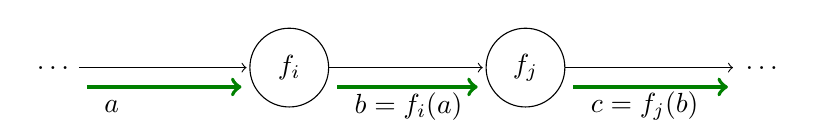
\begin{tikzpicture}[shorten >=1pt]
      	\tikzstyle{unit}=[draw,shape=circle,minimum size =1cm]

		\node (start) at (0,1){$\ldots$};
       	\node[unit](i) at (3,1){$f_i$};
        	\node[unit](j) at (6,1){$f_j$};
        	\node (end) at (9,1){$\ldots$};

        	\draw[->] (i) -- (j);
        	\draw[->] (start) -- (i);
        	\draw[->] (j) -- (end);
		
		\begin{scope}[transform canvas={yshift=-.7em}]
		\draw [->, Green, line width=0.05cm, shorten <=1mm, shorten >=1mm] (start) -- node {} (i);
  		\draw [->, Green, line width=0.05cm, shorten <=1mm, shorten >=1mm] (i) -- node {} (j);
  		\draw [->, Green, line width=0.05cm, shorten <=1mm, shorten >=1mm] (j) -- node {} (end);
		\end{scope}
		
		\begin{scope}[transform canvas={yshift=-1.4em}]
		\node (i-in) [right=0.2cm of start] {$a$};
		\node (j-in) [right=0.2cm of i] {$b=f_i(a)$};
		\node (j-out) [right=0.2cm of j] {$c=f_j(b)$};
		\end{scope}
\end{tikzpicture}
\end{center}
\end{frame}

\begin{frame}
{Backward pass}
\begin{itemize}
\item Order nodes in \textbf{reverse topological order} (every node appears after its children)
\item For each node, compute the partial derivative of its output w.r.t. its input, multiplied by the partial derivative of its children (chain rule)
\item Backward pass at intermediate node $f_i$:
\end{itemize}
\begin{center}
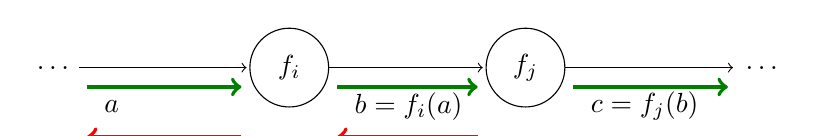
\begin{tikzpicture}[shorten >=1pt]
      	\tikzstyle{unit}=[draw,shape=circle,minimum size =1cm]

		\node (start) at (0,1){$\ldots$};
       	\node[unit](i) at (3,1){$f_i$};
        	\node[unit](j) at (6,1){$f_j$};
        	\node (end) at (9,1){$\ldots$};

        	\draw[->] (i) -- (j);
        	\draw[->] (start) -- (i);
        	\draw[->] (j) -- (end);
		
		\begin{scope}[transform canvas={yshift=-.7em}]
		\draw [->, Green, line width=0.05cm, shorten <=1mm, shorten >=1mm] (start) -- node {} (i);
  		\draw [->, Green, line width=0.05cm, shorten <=1mm, shorten >=1mm] (i) -- node {} (j);
  		\draw [->, Green, line width=0.05cm, shorten <=1mm, shorten >=1mm] (j) -- node {} (end);
		\end{scope}
		
		\begin{scope}[transform canvas={yshift=-1.4em}]
		\node (i-in) [right=0.2cm of start] {$a$};
		\node (j-in) [right=0.2cm of i] {$b=f_i(a)$};
		\node (j-out) [right=0.2cm of j] {$c=f_j(b)$};
		\end{scope}
		
		\begin{scope}[transform canvas={yshift=-2.5em}]
		\draw [<-, red, line width=0.05cm, shorten <=1mm, shorten >=1mm] (start) -- node {} (i);
  		\draw [<-, red, line width=0.05cm, shorten <=1mm, shorten >=1mm] (i) -- node {} (j);
%  		\draw [<-, red, line width=0.05cm, shorten <=1mm, shorten >=1mm] (j) -- node {} (end);
		\end{scope}
		
		\begin{scope}[transform canvas={yshift=-3.4em}]
		\node (i-out) [left=0.2cm of i] {$g_i=g_j \cdot \frac{\partial b}{\partial a} = \frac{\partial J}{\partial a}$};
		\node (j-out) [left=0.2cm of j] {$g_j=\frac{\partial J}{\partial b}$};
		\end{scope}
\end{tikzpicture}
\end{center}
\end{frame}

\begin{frame}{Multiple children}
\begin{itemize}
\item First sum partial derivatives from all children, then multiply.
\begin{columns}[c]

\column{.45\textwidth}

\includegraphics[width=1\columnwidth]{figures/backprop-general-node}

\pause{}

\column{.5\textwidth}
\begin{itemize}
\item Backprop for node $f$:
\item \textbf{Input}: $\frac{\partial J}{\partial b^{(1)}},\ldots,\frac{\partial J}{\partial b^{(N)}}$
\\
(Partials w.r.t. inputs to all children)
\item \textbf{Output}: 
\begin{eqnarray*}
\frac{\partial J}{\partial b} & = & \sum_{k=1}^{N}\frac{\partial J}{\partial b^{(k)}}\\
\text{ }\frac{\partial J}{\partial a} & = & \frac{\partial J}{\partial b}\frac{\partial b}{\partial a}
\end{eqnarray*}
\end{itemize}
\end{columns}

\end{itemize}
\end{frame}
%
%

\begin{frame}{Why backward?}
\begin{itemize}
    \item<+-> We can write the gradient in terms of chain rule.
    \begin{align}
    y &= y(c(b(a)))\\
    \frac{\partial y}{\partial a} &= \frac{\partial b}{\partial a}\frac{\partial c}{\partial b}\frac{\partial y}{\partial c}\\
    \frac{\partial y}{\partial a} &= \frac{\partial b}{\partial a}\left(\frac{\partial c}{\partial b}\frac{\partial y}{\partial c}\right)\\
    \frac{\partial y}{\partial a} &= \left(\frac{\partial b}{\partial a}\frac{\partial c}{\partial b}\right)\frac{\partial y}{\partial c}
    \end{align}
    \item<+->  The reverse order (backprop) is faster since we have a scalar output and a vector input, and it works well on most neural networks.
    \item<+->  Forward order could be faster if we have a scalar input and a vector output (less memory).
    \item<+->  Optimal ordering = matrix chain ordering problem.
\end{itemize}
\end{frame}

\begin{frame}
{Non-convex optimization}
\begin{figure}
\includegraphics[height=0.7\textheight]{figures/convex_cost_function}
\end{figure}
\begin{itemize}
\item Left: convex loss function. Right: non-convex loss function.
\end{itemize}
\end{frame}

\begin{frame}
{Non-convex optimization: challenges}
\begin{columns}
\begin{column}{0.6\textwidth}
\begin{itemize}
\item What if we converge to a bad local minimum?
\begin{itemize}
\item Rerun with a different initialization
\end{itemize}
\pause
\item Hit a saddle point 
\begin{itemize}
\item Doesn't often happen with SGD 
\item Second partial derivative test
\end{itemize}
\pause
\item Flat region: low gradient magnitude
\begin{itemize}
\item Possible solution: use ReLU instead of sigmoid 
\end{itemize}
\pause
\item High curvature: large gradient magnitude
\begin{itemize}
\item Possible solutions: Gradient clipping, adaptive step sizes
\end{itemize}
\pause
\end{itemize}
\end{column}
\begin{column}{0.4\textwidth}
\begin{figure}
\includegraphics[width=0.8\columnwidth]{figures/saddle_point}
\end{figure}
\end{column}
\end{columns}
\let\thefootnote\relax\footnotetext{\tiny{Reference: Chris De Sa's slides (CS6787 Lecture 7).}}
\end{frame}

\begin{frame}{Learning rate}
\begin{itemize}
\item One of the most important hyperparameter.
\item Start with a higher learning rate then decay towards zero.
\pause
\item Classic theory: convergence guarantee for stochastic gradient descent. Otherwise the update step has a noise term dominated by the noise of data sample.
\item Other explanation: Loss surface, avoidance of local minima, avoidance of memorization of noisy samples
\pause
\item Learning rate decay (staircase 10x, cosine, etc.), speeds up convergence
\end{itemize}
\end{frame}

\begin{frame}{More in-depth topics}
\begin{itemize}
    \item<+-> Neural networks have been a popular machine learning model in the past decade, due to its learning capability.
    \item<+-> Today: MLP + SGD (backprop)
    \item<+-> Adding structures: weight-sharing, convolution, recurrent, residual connection, attention
    \item<+-> Learning conditioning: normalization, optimizers
    \item<+-> Learning tasks: generative modeling, 3D perception, planning \& control
    \item<+-> System: GPU/TPU, parallel computing, gradient aggregation
    \item<+-> Some topics covered in DS-GA 1008 Deep Learning
\end{itemize}
\end{frame}

\begin{frame}{A side note}
\begin{itemize}
    \item<+-> Backprop is used to train the overwhelming majority of neural nets today.
    \item<+-> Despite its practical success, backprop is believed to be neurally implausible.
    \item<+-> No evidence for biological signals analogous to error derivatives.
    \item<+-> Forward \& backward weights are tied in backprop.
    \item<+-> Backprop requires synchronous update (1 forward followed by 1 backward).
    \item<+-> Biologically plausible alternatives we know about learn much more slowly on computers.
\end{itemize}
\end{frame}

\begin{frame}
{Review}
\begin{itemize}
\item<+-> Backpropagation is an algorithm for computing the gradient (partial derivatives + chain rule) efficiently.
\item<+-> It is used in gradient descent optimization for neural networks.
\item<+-> Key idea: function composition and the chain rule
% \item Key idea: function composition and dynamic programming
\item<+-> In practice, we can use existing software packages, e.g. PyTorch (backpropagation, neural network building blocks, optimization algorithms etc.)
\end{itemize}
\end{frame}

\end{document}